% arara: clean: { files: [main.pdf] }
% arara: lualatex: { shell: true, interaction: nonstopmode }
% arara: lualatex: { shell: true, interaction: nonstopmode }
% arara: clean: { files: [main.aux,main.bbl,main.blg,main.log,main.out,main.nav,main.snm,main.vrb,main.run.xml,main.toc,main-blx.bib] }

\documentclass[hyperref={pdfpagelabels=false},xcolor={dvipsnames},compress,onlytextwidth]{beamer}
\setbeamertemplate{navigation symbols}{}
\usepackage{lmodern}
\usepackage{svg}
\usepackage{listings}
\usepackage{url}
\usepackage[absolute,overlay]{textpos}
\usepackage{fontawesome}
\usepackage{fancyqr}
\usepackage{caption}
\IfFileExists{xcolor.sty}{
    \RequirePackage{xcolor}
}{
    \RequirePackage{color}
}
\usepackage{subfigure}
\usepackage{graphicx}
\usepackage{fontspec}

\newcommand{\source}[1]{\caption*{\tiny source: {#1}} }

\newfontfamily\jbmono{jetbrainsmono}[Path,
    Extension = .ttf,
    Contextuals = {Alternate},
    NFSSFamily = jbmono,
    UprightFont = fonts/*-Regular,
    ItalicFont = fonts/*-Italic,
    BoldFont = fonts/*-Bold,
    BoldItalicFont = fonts/*-BoldItalic,
    FontFace = {sb}{n}{fonts/*-Medium},
    FontFace = {sb}{it}{fonts/*-MediumItalic},
    FontFace = {eb}{n}{fonts/*-ExtraBold},
    FontFace = {eb}{it}{fonts/*-ExtraBoldItalic}
]

\lstdefinestyle{kotlin}
{
    basicstyle=\linespread{1.15}\jbmono\tiny,
    emph={filter, first, firstOrNull, forEach, lazy, map,fold, mapNotNull, println, until, downTo, TODO},
    keywords={!in, !is, abstract, actual, annotation, as, as?, break, by, catch, value, class, companion, const, constructor, continue, crossinline, data, delegate, do, dynamic, else, enum, expect, external, false, field, file, final, finally, for, fun, get, if, import, in, infix, init, inner, interface, internal, is, lateinit, noinline, null, object, open, operator, out, override, package, param, private, property, protected, public, receiveris, reified, return, return@, sealed, set, setparam, super, suspend, tailrec, this, throw, true, try, typealias, typeof, val, var, vararg, when, where, while},
    ndkeywords={@Deprecated, @JvmField, @JvmInline, @JvmName, @JvmOverloads, @JvmStatic, @JvmSynthetic, Array, Byte, UByte, Double, Float, Int, UInt, Integer, Iterable, Long, Runnable, Short, String, Any, Unit, Nothing},
    comment=[l]{//},
    morecomment=[s]{/*}{*/},
    morestring=[b]",
    morestring=[s]{"""*}{*"""},
    escapeinside={\%*}{*)},
    captionpos=b,
    sensitive=true,
    breakatwhitespace=true,
    breaklines=true,
    prebreak=\raisebox{0ex}[0ex][0ex]{\ensuremath{\hookleftarrow}},
    numbers=left,
    stepnumber=1,
    numberstyle=\linespread{1.15}\jbmono\tiny,
}

\definecolor{keyword}{HTML}{BA2CA3}
\definecolor{ndkeyword}{HTML}{3D85C6}
\definecolor{string}{HTML}{4BAB22}
\definecolor{comment}{HTML}{999999}

\lstset{
    inputencoding=utf8,
    extendedchars=\true,
    showstringspaces=false,
    columns=fullflexible,
    keepspaces=true,
    keywordstyle=\color{keyword},
    ndkeywordstyle=\color{ndkeyword},
    stringstyle=\color{string},
    commentstyle=\color{comment},
    style=kotlin
}
\usetheme{Berlin}

\AtBeginSection[]{
    \begin{frame}
        \vfill
        \centering
        \begin{beamercolorbox}[sep=8pt,center,shadow=false,rounded=false]{title}
            \usebeamerfont{title}\insertsectionhead\par%
        \end{beamercolorbox}
        \vfill
    \end{frame}
}

\title{Deep dive into coroutines}
\subtitle{on the example of Kotlin implementation}
\author{Maciej Procyk}
\date{
\includegraphics[width=75pt]{images/happy}\\March 27, 2023}
\begin{document}

    \logo{\includesvg[width=30pt]{images/logo.svg}}

    {
        \setbeamertemplate{logo}{}
        \setbeamertemplate{headline}{}
        \begin{frame}
            \maketitle
        \end{frame}
    }

    \begin{frame}
        \frametitle{Table of contents}
        \tableofcontents
    \end{frame}


    \section{Introduction}

    \subsection{Main ideas}

    \begin{frame}{General description}
        \begin{itemize}
            \item described as ``functions whose execution you can pause''\pause
            \item computation can be paused and resumed without blocking a thread\pause
            \item generalization of subroutines for cooperative multitasking\pause
            \item fast context switching\pause
            \item perfect tool for implementing iterators, infinite lists, pipes\pause
            \item asynchronous code in synchronous manner
        \end{itemize}
    \end{frame}

    \begin{frame}{Fundamental characteristics}
        \begin{enumerate}
            \item the values of data local to a coroutine persist between successive calls\pause
            \item the execution of a coroutine is suspended as control leaves it, only to carry on where it left off when control re-enters the coroutine at some later stage
        \end{enumerate}
    \end{frame}

    \subsection{Practical background}

    \begin{frame}{Asynchronous programming}
        \begin{itemize}
            \item nowadays, we write the programs that wait for a lot of time\pause
            \item we write them using threads, but there are a few limitations\pause
            \item the number of threads cannot be too high, as they consume a lot of memory\pause
            \item e.g.\ on Linux x64 default stack size (configured with \texttt{-XX:ThreadStackSize} or \texttt{-Xss} option) is 256 KB\pause
            \item which means that 100K threads would consume about 24 GB of memory\pause
            \item that's a lot and what if we think about 1M threads
        \end{itemize}
    \end{frame}

    \begin{frame}{Coroutines vs threads}
        \begin{itemize}
            \item the difference is that threads are scheduled on cores preemptively, while coroutines are scheduled onto threads cooperatively\pause
            \item starting a thread on JVM requires starting native thread, which consumes memory for its stack\pause
            \item switching between threads requires going through system's kernel\pause
            \item and is expensive in terms of CPU cycles consumed during that operation
        \end{itemize}
    \end{frame}

    \begin{frame}{Coroutines vs threads}
        \begin{itemize}
            \item coroutine is user-level abstraction (implemented by the language compiler in case of Kotlin)\pause
            \item in the simplest case it's a single reference object in JVM heap memory\pause
            \item switching between coroutines is as simple (and cheap) as invoking a regular function
        \end{itemize}
    \end{frame}

    \begin{frame}[fragile]{Sample code starting 100 000 threads}
        \lstinputlisting[style=kotlin,firstline=7,lastline=16]{../kotlin-coroutines-samples/src/main/kotlin/introduction/ManyThreads.kt}\pause
        \begin{itemize}
            \item possible, but takes a lot of time (and actually they don't exist in the same time)\pause
            \item if we increase the sleep time the number of threads existing in the same time would increase\pause
            \item and we would end up with \texttt{Exception in thread "main" java.lang.OutOfMemoryError ...}
        \end{itemize}
    \end{frame}

    \begin{frame}[fragile]{Sample code starting 100 000 jobs}
        \lstinputlisting[style=kotlin,firstline=8,lastline=17]{../kotlin-coroutines-samples/src/main/kotlin/introduction/ManyCoroutines.kt}\pause
        \begin{itemize}
            \item explicitly defined context is needed to start the whole process\pause
            \item code runs over 10 times faster than the threads implementation\pause
            \item because it uses computer resources more thoughtful
        \end{itemize}
    \end{frame}

    \begin{frame}[fragile]{Toy problem wasting computer resources on sleeping}
        \lstinputlisting[style=kotlin,firstline=5,lastline=9]{../kotlin-coroutines-samples/src/main/kotlin/introduction/ToyProblem.kt}\pause
        \begin{itemize}
            \item potentially, the application may have thousands of these tasks run concurrently\pause
            \item but every of them would consume a single thread to be executed\pause
            \item the problem are the blocking functions which are related to IO operations and expensive processing
        \end{itemize}
    \end{frame}

    \begin{frame}[fragile]{The ``old'' JVM solution for this problem are callbacks}
        \lstinputlisting[style=kotlin,firstline=5,lastline=11]{../kotlin-coroutines-samples/src/main/kotlin/introduction/ToyProblemCallbacks.kt}\pause
        \begin{itemize}
            \item functions returns immediately and run the callbacks later to get the result\pause
            \item this introduces ``callback hell'' problem\pause
            \item this code has multiple limitations - the structure of code prevents imperative coding (how to write loops?)
        \end{itemize}
    \end{frame}

    \begin{frame}[fragile]{Writing imperative code with callbacks}
        \only<1>{\lstinputlisting[style=kotlin,firstline=3,lastline=8]{../kotlin-coroutines-samples/src/main/kotlin/introduction/LoopExample.kt}}
        \only<2->{\lstinputlisting[style=kotlin,firstline=10,lastline=20]{../kotlin-coroutines-samples/src/main/kotlin/introduction/LoopExample.kt}}
        \begin{itemize}
            \item<3-> hard to understand intention of programmer using callbacks
            \item<4-> additionally, there's extra cost related to working with the references for callbacks
            \item<5-> this solution doesn't scale well so other approach needs to be found
        \end{itemize}
    \end{frame}

    \begin{frame}[fragile]{Futures/Promises/Rx being a rescue?}
        \lstinputlisting[style=kotlin,firstline=8,lastline=15]{../kotlin-coroutines-samples/src/main/kotlin/introduction/ToyProblemRx.kt}\pause
        \begin{itemize}
            \item we got nicer, composable code, with no extra indentation\pause
            \item we're able to propagate our exceptions\pause
            \item but the combinators are the problem - it might be hard to learn them all\pause
            \item while there are different libraries with other names
        \end{itemize}
    \end{frame}

    \begin{frame}[fragile]{Kotlin solution are coroutines}
        \lstinputlisting[style=kotlin,firstline=10,lastline=14]{../kotlin-coroutines-samples/src/main/kotlin/introduction/ToyProblemCoroutines.kt}\pause
        \begin{itemize}
            \item need to mark functions with \texttt{suspend} modifier\pause
            \item but the structure of the code looks like regular code (loops, exceptions, extension functions)\pause
            \item we got ``not obvious'' suspension points\pause
            \item but the good IDE helps here a lot if we're interested in this
        \end{itemize}
    \end{frame}


    \section{Coroutines in details}

    \subsection{Implementation details}

    \begin{frame}[fragile]{What's under the hood?}
        \begin{itemize}
            \item suspending functions are implemented via Continuation-Passing-Style (CPS)\pause
            \item every suspending function has an additional \texttt{Continuation} parameter passed implicitly when function is invoked\pause
            \item consider the following signature of \texttt{suspend} function\pause
        \end{itemize}
        \lstinputlisting[style=kotlin,firstline=10,lastline=10,numbers=none]{../kotlin-coroutines-samples/src/main/kotlin/details/CPS.kt}\pause
        \begin{itemize}
            \item its actual implementation after compiler transformation has the following form\pause
        \end{itemize}
        \lstinputlisting[style=kotlin,firstline=19,lastline=19,numbers=none]{../kotlin-coroutines-samples/src/main/kotlin/details/CPS.kt}
    \end{frame}

    \begin{frame}[fragile]{Continuation interface}
        \begin{itemize}
            \item<1-> \texttt{context} represents an arbitrary user-defined context that is associated with the coroutine
            \item<2-> \texttt{resumeWith} function is a completion callback that is used to report on coroutine completion:
            \begin{itemize}
                \item<3-> a success - with a value
                \item<4-> a failure - with an exception
            \end{itemize}
            \item<5-> there are two extension functions defined for convenience
        \end{itemize}
        \visible<1->{\lstinputlisting[style=kotlin,firstline=5,lastline=8]{../kotlin-coroutines-samples/src/main/kotlin/details/ContinuationInterface.kt}}
        \visible<5->{\lstinputlisting[style=kotlin,firstline=10,lastline=12]{../kotlin-coroutines-samples/src/main/kotlin/details/ContinuationInterface.kt}}
    \end{frame}

    \begin{frame}[fragile]{How the typical implementation looks like?}
        \only<1>{\lstinputlisting[style=kotlin,firstline=10,lastline=16]{../kotlin-coroutines-samples/src/main/kotlin/details/CPS.kt}}
        \only<2->{\lstinputlisting[style=kotlin,firstline=21,lastline=31]{../kotlin-coroutines-samples/src/main/kotlin/details/CPS.kt}}
        \begin{itemize}
            \item<3-> we use the callback interface to resume the continuation\pause
            \item<4-> to actually suspend execution function must invoke other suspending function - \texttt{await} implementation invokes a suspending function \texttt{suspendCoroutine}
        \end{itemize}
    \end{frame}

    \begin{frame}[fragile]{State machines as perfect solution}
        \begin{itemize}
            \item it's crucial to implement coroutines efficiently, i.e.\ create as few classes and objects as possible\pause
            \item compiler creates a single instance of class that may have any number of suspension points\pause
            \item general idea - suspending function is a state machine\pause
            \item states corresponds to suspension points\pause
        \end{itemize}
        \lstinputlisting[style=kotlin,firstline=9,lastline=15]{../kotlin-coroutines-samples/src/main/kotlin/details/StateMachine.kt}
    \end{frame}

    \begin{frame}[fragile]{State machines as perfect solution}
        \begin{itemize}
            \item three states for the given block of code:\pause
            \begin{enumerate}
                \item initial (before any suspension point)\pause
                \item after the first suspension point\pause
                \item after the second suspension point\pause
            \end{enumerate}
            \item each of them being an entry point to continuation of this block\pause
            \item which can be seen as \texttt{switch} statement with label to each suspension point\pause
            \item the execution is continued with \texttt{resumeWith} method of coroutine which selects the current branch\pause
            \item local variables are generated as class fields of anonymous class
        \end{itemize}
    \end{frame}

    \begin{frame}[fragile]{State machines implementation}
        Pseudo-code corresponding to JVM bytecode created for suspending function:
        \lstinputlisting[language=Java,firstline=1,lastline=14]{code/state_machine.jvm}
    \end{frame}
    \begin{frame}[fragile]{State machines implementation}
        \lstinputlisting[language=Java,firstline=15,lastline=36,firstnumber=15]{code/state_machine.jvm}
    \end{frame}

    \begin{frame}[fragile]{Generators}
        \begin{itemize}
            \item generators with \texttt{yield} can be easily implemented using \texttt{suspend} functions\pause
            \item and that's how the Kotlin std-lib does, providing \texttt{Sequence<T>} abstraction with \texttt{yield} as a function of \texttt{SequenceScope<T>}\pause
            \item they can represent potentially infinite lists (like in Haskell)\pause
            \item or just in general lazily computed sequences\pause
            \item the strength of them is supporting arbitrary control flow, with \texttt{for}, \texttt{when}, \texttt{try}/\texttt{catch} etc.
        \end{itemize}
    \end{frame}

    \begin{frame}[fragile]{Generators - example Fibonacci sequence}
        \lstinputlisting[style=kotlin,firstline=5,lastline=15]{../kotlin-coroutines-samples/src/main/kotlin/details/Generators.kt}\pause
        \lstinputlisting[style=kotlin,firstline=3,lastline=3,numbers=none]{../kotlin-coroutines-samples/src/main/kotlin/details/Generators.kt}
    \end{frame}

    \subsection{Fundamental concepts}

    \begin{frame}[fragile]{Initial idea - extra DSL}
        \lstinputlisting[style=kotlin,firstline=13,lastline=17]{../kotlin-coroutines-samples/src/main/kotlin/details/InitialIdea.kt}\pause
        \begin{itemize}
            \item original prototype defined the library functions, similar to keywords from e.g.\ C\#, Typescript, Dart, Python\pause
            \item but the compiler needed to know that \texttt{await} can be suspended, so it was marked with \texttt{suspend} modifier\pause
            \item so the decision was to remove the need for \texttt{await} call\pause
            \item which led to adding \texttt{suspend} modifier to functions instead of using \texttt{async} builder
        \end{itemize}
    \end{frame}

    \begin{frame}[fragile]{Initial idea - extra DSL}
        \begin{itemize}
            \item there was some fear as no other language resigned from \texttt{async}/\texttt{await}\pause
            \item actually in Go language nobody is worried about the not visible suspension points\pause
        \end{itemize}
        \begin{columns}
            \begin{column}{0.5\textwidth}
                \lstinputlisting[style=kotlin,firstline=12,lastline=15]{../kotlin-coroutines-samples/src/main/kotlin/details/LikeGoSolution.kt}\pause
            \end{column}
            \begin{column}{0.5\textwidth}
                \lstinputlisting[style=kotlin,firstline=17,lastline=20]{../kotlin-coroutines-samples/src/main/kotlin/details/LikeGoSolution.kt}\pause
            \end{column}
        \end{columns}
        \lstinputlisting[style=kotlin,firstline=22,lastline=27]{../kotlin-coroutines-samples/src/main/kotlin/details/LikeGoSolution.kt}
    \end{frame}

    \begin{frame}[fragile]{Context and Scope of execution}
        \only<1-5>{\lstinputlisting[style=kotlin,firstline=12,lastline=15]{../kotlin-coroutines-samples/src/main/kotlin/details/ContextAndScope.kt}}
        \only<6->{\lstinputlisting[style=kotlin,firstline=17,lastline=21]{../kotlin-coroutines-samples/src/main/kotlin/details/ContextAndScope.kt}}
        \begin{itemize}
            \item<2-> coroutines execute in some context represented by the \texttt{CoroutineContext} type
            \item<3-> it contains the \texttt{CoroutineDispatcher} which delegates the coroutine to some thread of execution
            \item<4-> it's inherited from the parent \texttt{CoroutineScope} by default
            \item<5-> and all coroutine builders like \texttt{launch} and \texttt{async} accept optional \texttt{CoroutineContext} to explicitly specify the dispatcher for the new coroutine context
        \end{itemize}
    \end{frame}

    \subsection{Structured concurrency}

    \begin{frame}[fragile]{What is structured concurrency?}
        \begin{columns}
            \begin{column}{0.68\textwidth}
                \begin{itemize}
                    \item<1-> compare understanding concurrency to understanding program control flow
                    \item<2-> with \texttt{goto} instruction it can start being hard to understand
                    \item<3-> but when we limit ourselves to known structures, it's much more obvious and not that limited
                    \item<4-> in concurrent programming model we have the same problem with tasks
                    \item<5-> introducing some ``structures'' to keep everything in consistent state helps in understanding what may happen
                \end{itemize}
            \end{column}
            \begin{column}{0.28\textwidth}
                \only<2>{
                    \begin{figure}
                        \centering
                        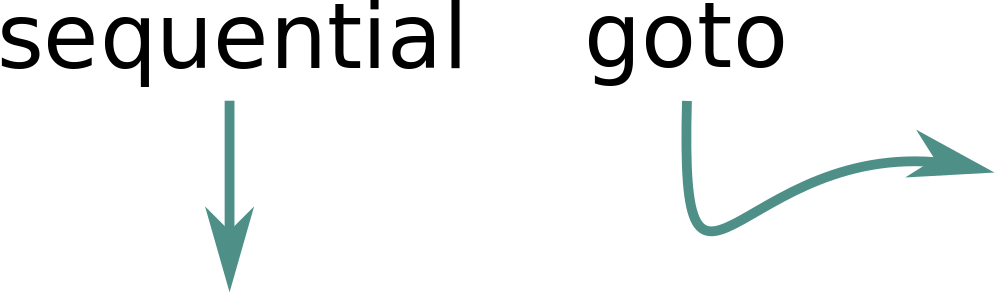
\includegraphics[width=80pt]{images/unstrucutred-code}
                        \source{https://vorpus.org/blog/notes-on-structured-concurrency-or-go-statement-considered-harmful/}
                    \end{figure}
                }
                \only<3>{
                    \begin{figure}
                        \centering
                        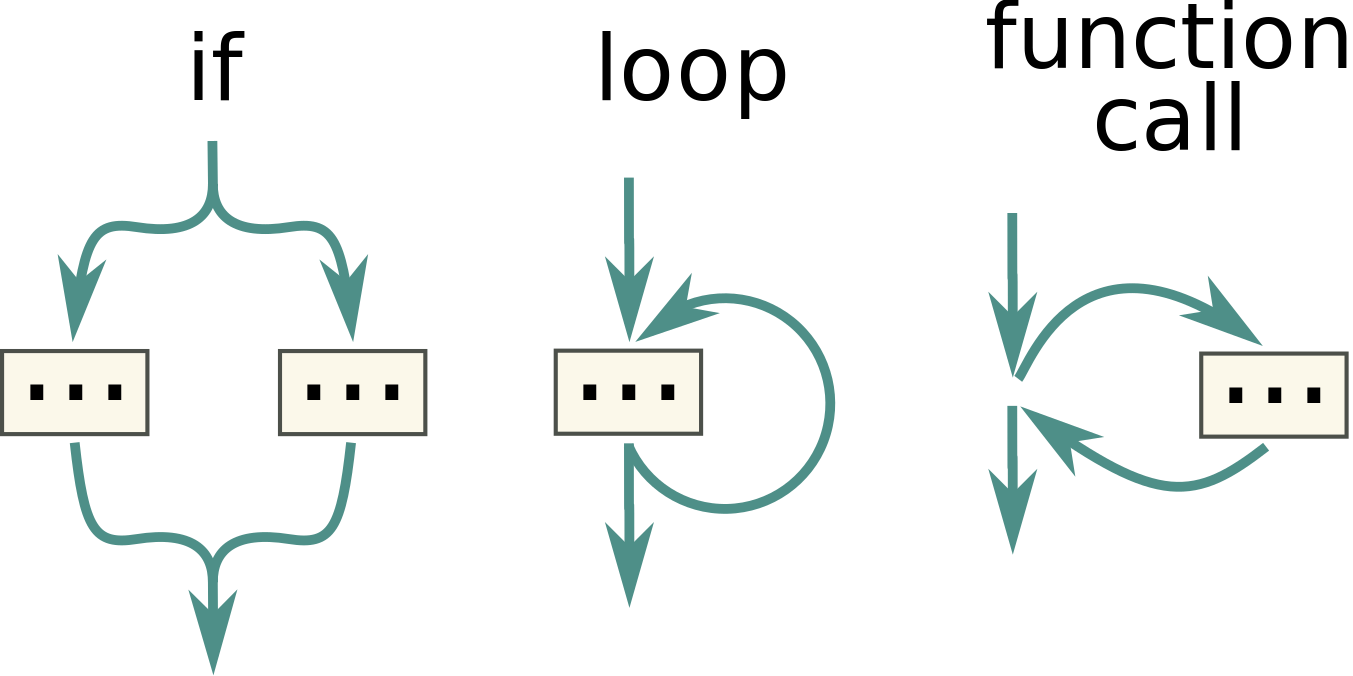
\includegraphics[width=80pt]{images/strucutred-code}
                        \source{https://vorpus.org/blog/notes-on-structured-concurrency-or-go-statement-considered-harmful/}
                    \end{figure}
                }
                \only<5->{
                    \begin{figure}
                        \centering
                        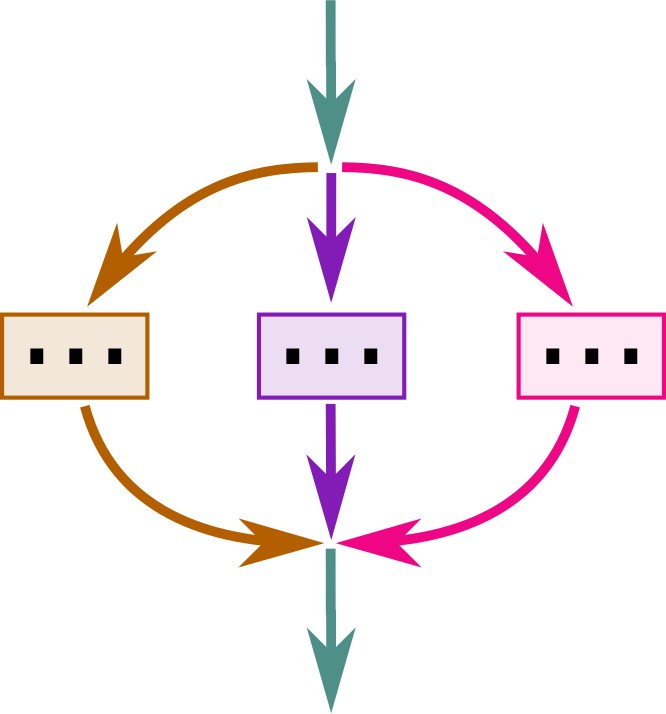
\includegraphics[width=80pt]{images/structured-concurrency}
                        \source{https://vorpus.org/blog/notes-on-structured-concurrency-or-go-statement-considered-harmful/}
                    \end{figure}
                }
            \end{column}
        \end{columns}
    \end{frame}

    \begin{frame}[fragile]{\texttt{launch} and \texttt{async} coroutine builders}
        \begin{itemize}
            \item \texttt{launch} produces a \texttt{Job}, while \texttt{async} produces a \texttt{Deferred<T>}\pause
            \item they start a new coroutine without blocking the current one\pause
            \item they can be called only in context of some \texttt{CoroutineScope} which is ``responsible'' for its execution\pause
            \item coroutine is cancelled when the returned \texttt{Job} is cancelled\pause
            \item but still we need to manually check for cancellation in long-running tasks
        \end{itemize}
    \end{frame}

    \begin{frame}[fragile]{Structured concurrency in Kotlin}
        \begin{itemize}
            \item \texttt{CoroutineScope} can be seen a structure in which the control flows of concurrent tasks are merged\pause
            \item \texttt{launch} and \texttt{async} corresponds to creating new execution branches\pause
            \item parent always waits for children completion\pause
            \item there's no place for loosing some resource\pause
            \item there's no exception lost - they're propagated
        \end{itemize}
    \end{frame}

    \begin{frame}[fragile]{\texttt{launch} running examples}
        \lstinputlisting[style=kotlin,firstline=13,lastline=16]{../kotlin-coroutines-samples/src/main/kotlin/details/LaunchDetails.kt}\pause
        \begin{itemize}
            \item executes \texttt{sayA} and \texttt{sayB} sequentially\pause
            \item finishes \texttt{justSuspensionPoints} when both jobs are finished
        \end{itemize}
    \end{frame}

    \begin{frame}[fragile]{\texttt{launch} running examples}
        \lstinputlisting[style=kotlin,firstline=18,lastline=21]{../kotlin-coroutines-samples/src/main/kotlin/details/LaunchDetails.kt}\pause
        \begin{itemize}
            \item executes \texttt{sayA} and \texttt{sayB} concurrently\pause
            \item finishes \texttt{launchFirstInScope} when both jobs are finished
        \end{itemize}
    \end{frame}

    \begin{frame}[fragile]{\texttt{launch} running examples}
        \lstinputlisting[style=kotlin,firstline=23,lastline=26]{../kotlin-coroutines-samples/src/main/kotlin/details/LaunchDetails.kt}\pause
        \begin{itemize}
            \item executes \texttt{sayA} and \texttt{sayB} concurrently\pause
            \item finishes \texttt{launchBothInScope} when both jobs are finished
        \end{itemize}
    \end{frame}

    \begin{frame}[fragile]{\texttt{launch} running examples}
        \lstinputlisting[style=kotlin,firstline=28,lastline=31]{../kotlin-coroutines-samples/src/main/kotlin/details/LaunchDetails.kt}\pause
        \begin{itemize}
            \item executes \texttt{sayA} and \texttt{sayB} concurrently\pause
            \item when \texttt{sayA} fails, \texttt{sayB} is cancelled as well
        \end{itemize}
    \end{frame}

    \begin{frame}[fragile]{\texttt{launch} running examples}
        \lstinputlisting[style=kotlin,firstline=33,lastline=36]{../kotlin-coroutines-samples/src/main/kotlin/details/LaunchDetails.kt}\pause
        \begin{itemize}
            \item executes \texttt{sayA} and \texttt{sayB} concurrently\pause
            \item when \texttt{sayA} fails, \texttt{sayB} is executed until it finishes
        \end{itemize}
    \end{frame}

    \begin{frame}[fragile]{Higher-order function}
        \begin{itemize}
            \item introducing coroutine brings advantage of no extra need for higher-order combinators like \texttt{flatMap}\pause
            \item it's enough to use the \texttt{suspend} modifier for lambda parameter\pause
        \end{itemize}
        \lstinputlisting[style=kotlin,firstline=7,lastline=18]{../kotlin-coroutines-samples/src/main/kotlin/details/HigherOrderFunctions.kt}
    \end{frame}


    \section{Higher-level APIs}

    \subsection{Main ideas}

    \begin{frame}[fragile]{\texttt{Channel<T>} in Kotlin}
        \only<1-2>{
            \begin{itemize}
                \item<1-> is implemented in Kotlin as a library, conceptually very similar to \texttt{BlockingQueue}
                \item<2-> implements \texttt{SendChannel<T>} and \texttt{ReceiveChannel<T>}
            \end{itemize}
            \only<2>{\lstinputlisting[style=kotlin,firstline=140,lastline=148]{../kotlin-coroutines-samples/src/main/kotlin/details/Channels.kt}}
        }
        \only<3->{
            \begin{itemize}
                \item<1-> is implemented in Kotlin as a library, conceptually very similar to \texttt{BlockingQueue}
                \item<2-> implements \texttt{SendChannel<T>} and \texttt{ReceiveChannel<T>}
                \item<3-> \texttt{send} suspends when the channel buffer is full, while \texttt{receive} suspends when the buffer is empty
                \item<4-> channels are hot - there's a coroutine on the other side of the channel that produces values, so we cannot just drop a reference to the ReceiveChannel, because the producer is going to be suspended forever waiting for a consumer, wasting memory resources, open network connections, etc.
            \end{itemize}
        }
    \end{frame}

    \begin{frame}[fragile]{\texttt{Flow<T>} in Kotlin}
        \begin{itemize}
            \item<1-> represents the stream of values that are being computed asynchronously
            \item<2-> can be used just like a Sequence<T> type for synchronously computed values
            \item<3-> flows are cold streams similar to sequences
            \item<4-> the code inside a flow builder does not run until the flow is collected
        \end{itemize}
    \end{frame}

    \subsection{Practical example}



    \begin{frame}[fragile]{Images downloader - goals}
        \begin{itemize}
            \item have single abstraction responsible for caching the results\pause
            \item have multiple workers responsible for doing the job\pause
            \item communicate between these abstractions in safely way\pause
            \item structure our concurrency model to be sure what's going on
        \end{itemize}
    \end{frame}

    \begin{frame}[fragile]{Images downloader - downloader}
        \lstinputlisting[style=kotlin,firstline=45,lastline=66]{../kotlin-coroutines-samples/src/main/kotlin/details/Channels.kt}
    \end{frame}

    \begin{frame}[fragile]{Images downloader - worker}
        \lstinputlisting[style=kotlin,firstline=68,lastline=79]{../kotlin-coroutines-samples/src/main/kotlin/details/Channels.kt}
    \end{frame}

    \begin{frame}[fragile]{Images downloader - common scope}
        \lstinputlisting[style=kotlin,firstline=35,lastline=43]{../kotlin-coroutines-samples/src/main/kotlin/details/Channels.kt}
    \end{frame}

    \begin{frame}[fragile]{Images downloader - Jetpack Compose demo}
        \lstinputlisting[style=kotlin,firstline=86,lastline=91]{../kotlin-coroutines-samples/src/main/kotlin/details/Channels.kt}
    \end{frame}

    \section*{Appendix}
    \subsection*{Resources}

    \begin{frame}{Still confused? Check out these places}
        \begin{enumerate}
            \item Roman Elizarov - Structured concurrency \href{https://www.youtube.com/watch?v=Mj5P47F6nJg}{\beamergotobutton{Watch}}
            \item KotlinConf 2017 - Introduction to Coroutines by Roman Elizarov \href{https://www.youtube.com/watch?v=_hfBv0a09Jc}{\beamergotobutton{Watch}}
            \item KotlinConf 2017 - Deep Dive into Coroutines on JVM by Roman Elizarov \href{https://www.youtube.com/watch?v=YrrUCSi72E8}{\beamergotobutton{Watch}}
            \item KotlinConf 2018 - Kotlin Coroutines in Practice by Roman Elizarov \href{https://www.youtube.com/watch?v=a3agLJQ6vt8}{\beamergotobutton{Watch}}
            \item KotlinConf 2019 - Asynchronous Data Streams with Kotlin Flow by Roman Elizarov \href{https://www.youtube.com/watch?v=tYcqn48SMT8}{\beamergotobutton{Watch}}
            \item Notes on structured concurrency, or: Go statement considered harmful \href{https://web.archive.org/web/20230315053056/https://vorpus.org/blog/notes-on-structured-concurrency-or-go-statement-considered-harmful/}{\beamergotobutton{Read}}
            \item Revisiting Coroutines, Ana Moura \& Roberto Ierusalimschy \href{https://web.archive.org/web/20230128095928/http://www.inf.puc-rio.br/~roberto/docs/MCC15-04.pdf}{\beamergotobutton{Read}}
        \end{enumerate}
    \end{frame}

    {
        \setbeamertemplate{logo}{}
        \setbeamertemplate{headline}{}
        \begin{frame}{}
            \centering
            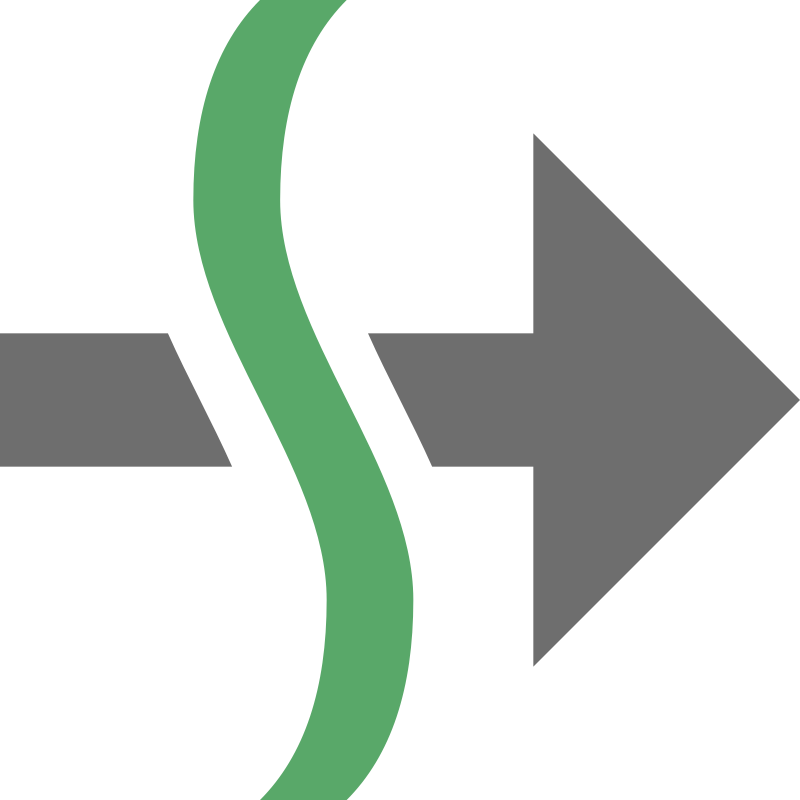
\includegraphics[width=100pt]{images/suspend}\\\vspace{1cm}
            \emph{\Large Time to \texttt{suspend}\\\vspace{0.6cm}Thank you for your attention!}
            \begin{textblock}{0.3}(0.7,10.5)
                \begin{figure}[h!]
                    \centering
                    \fancyqr[image=\small\faGithub,image padding=1,color=black!90!gray,height=30pt]{https://github.com/avan1235/kotlin-coroutines/}
                \end{figure}
            \end{textblock}
        \end{frame}
    }

\end{document}
